\documentclass[a4paper,12pt]{article}
\usepackage[utf8]{inputenc}
\usepackage{graphicx}
\usepackage{float}
\usepackage{booktabs}
\usepackage{geometry}
\usepackage{setspace}
\usepackage{caption}
\usepackage{hyperref}

\geometry{margin=1in}
\setstretch{1.2}

\begin{document}

\begin{titlepage}
    \centering
    \vspace*{3cm}
    {\Large\textbf{Individual Assignment: Matrix Multiplication}}\\[1cm]
    {\large Big Data}\\[0.5cm]
    {\large Grado en Ciencia e Ingeniería de Datos}\\[0.3cm]
    {\large Universidad de Las Palmas de Gran Canaria}\\[2cm]
    \textbf{Andrea Dumpierrez Medina}\\[0.5cm]
    \vfill
\end{titlepage}

\section*{Introduction}

This report presents a comparative study of matrix multiplication performance implemented in three different programming languages: Python, Java, and C. The purpose of this experiment is to analyze how execution time scales with the size of the input matrices, taking into account the efficiency of each language in handling computationally intensive operations.

Matrix multiplication is one of the most fundamental operations in scientific computing, machine learning, and data analysis. Its computational complexity is $O(n^3)$ in its basic implementation, meaning that performance is heavily influenced by both the efficiency of the programming language and the optimization of its libraries or compilers.

Benchmarking different implementations allows us to evaluate not only the raw computational performance of each language but also the trade-offs between development simplicity, readability, and execution speed.

\section*{Methodology}

Each program multiplies two randomly generated $n \times n$ matrices filled with floating-point numbers between 0 and 1. The same matrix sizes were tested across all implementations to ensure consistency in comparison. The experiments were repeated several times for each matrix size, and the average execution time was recorded.

The matrix sizes tested were: \textbf{10, 25, 50, 100, 200, 300, 400, 500, 700}.  
Each implementation was executed 7 times per matrix size to minimize fluctuations caused by external processes.

The results were stored in CSV format and visualized using benchmarking and plotting tools to provide a clearer view of performance differences.

\section*{Performance Metrics}

To evaluate the performance of the three implementations (Python, Java, and C), the following metrics were considered:

\begin{itemize}
    \item \textbf{Execution Time (s):} The time required to perform the matrix multiplication for each matrix size.
    \item \textbf{Memory Usage:} Although not measured explicitly, inferred based on the computational efficiency of each language.
    \item \textbf{CPU Usage (optional):} Observed qualitatively during testing, showing differences in thread optimization.
\end{itemize}

The main focus of this analysis is execution time, as it provides a direct measure of computational efficiency.

\section*{Results}

Table~\ref{tab:results} summarizes the average execution times for each language and matrix size.

\begin{table}[H]
    \centering
    \caption{Average execution time (s) for matrix multiplication across languages.}
    \label{tab:results}
    \begin{tabular}{cccc}
        \toprule
        \textbf{Matrix Size (n×n)} & \textbf{Python (s)} & \textbf{Java (s)} & \textbf{C (s)} \\
        \midrule
        10  & 0.0000  & 0.000026  & 0.000005 \\
        25  & 0.0000  & 0.000223  & 0.000041 \\
        50  & 0.0091  & 0.000245  & 0.000329 \\
        100 & 0.0616  & 0.000806  & 0.002599 \\
        200 & 0.4876  & 0.005167  & 0.021321 \\
        300 & 1.7318  & 0.024897  & 0.072499 \\
        400 & 4.2121  & 0.067373  & 0.173197 \\
        500 & 8.9297  & 0.142549  & 0.347377 \\
        700 & 32.9756 & 0.411627  & 0.927541 \\
        \bottomrule
    \end{tabular}
\end{table}

\section*{Graphical Analysis}

Figures~\ref{fig:linear}, \ref{fig:log}, and \ref{fig:bar} present the graphical analysis of the results. These visualizations allow for better comparison between programming languages.

\begin{figure}[H]
    \centering
    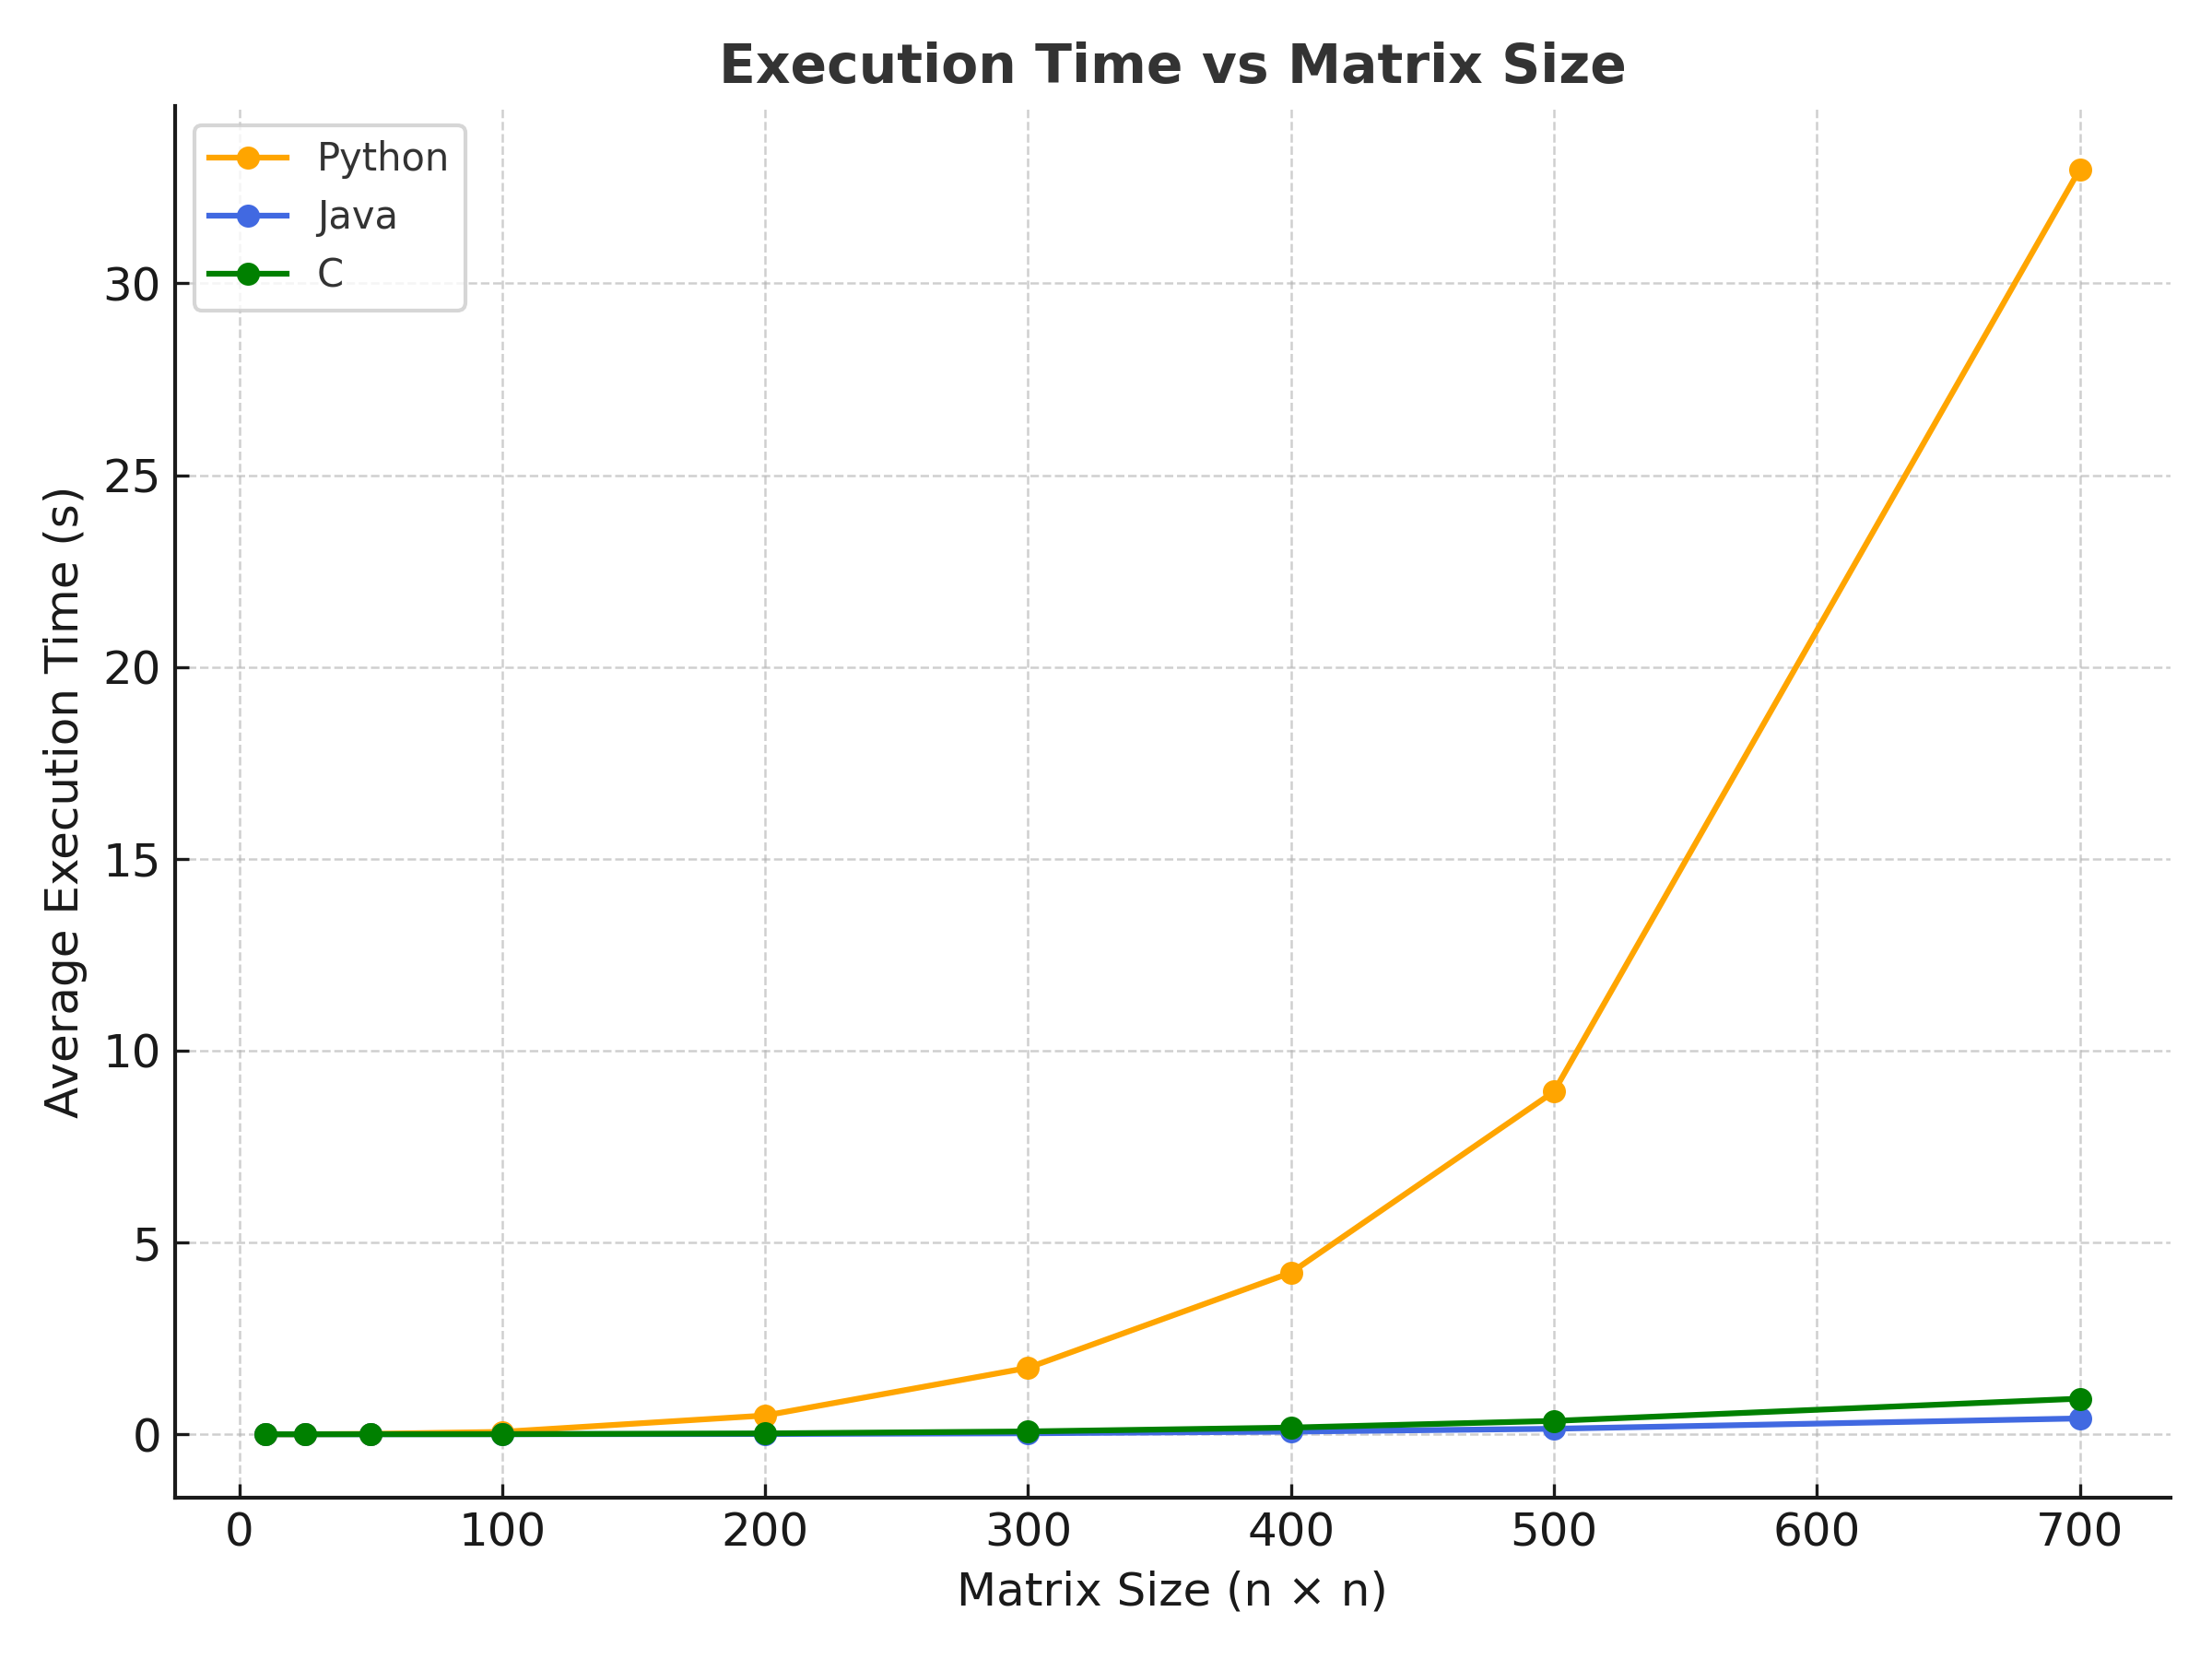
\includegraphics[width=0.85\textwidth]{execution_time_linear.png}
    \caption{Execution time comparison for Python, Java, and C implementations.}
    \label{fig:linear}
\end{figure}

\begin{figure}[H]
    \centering
    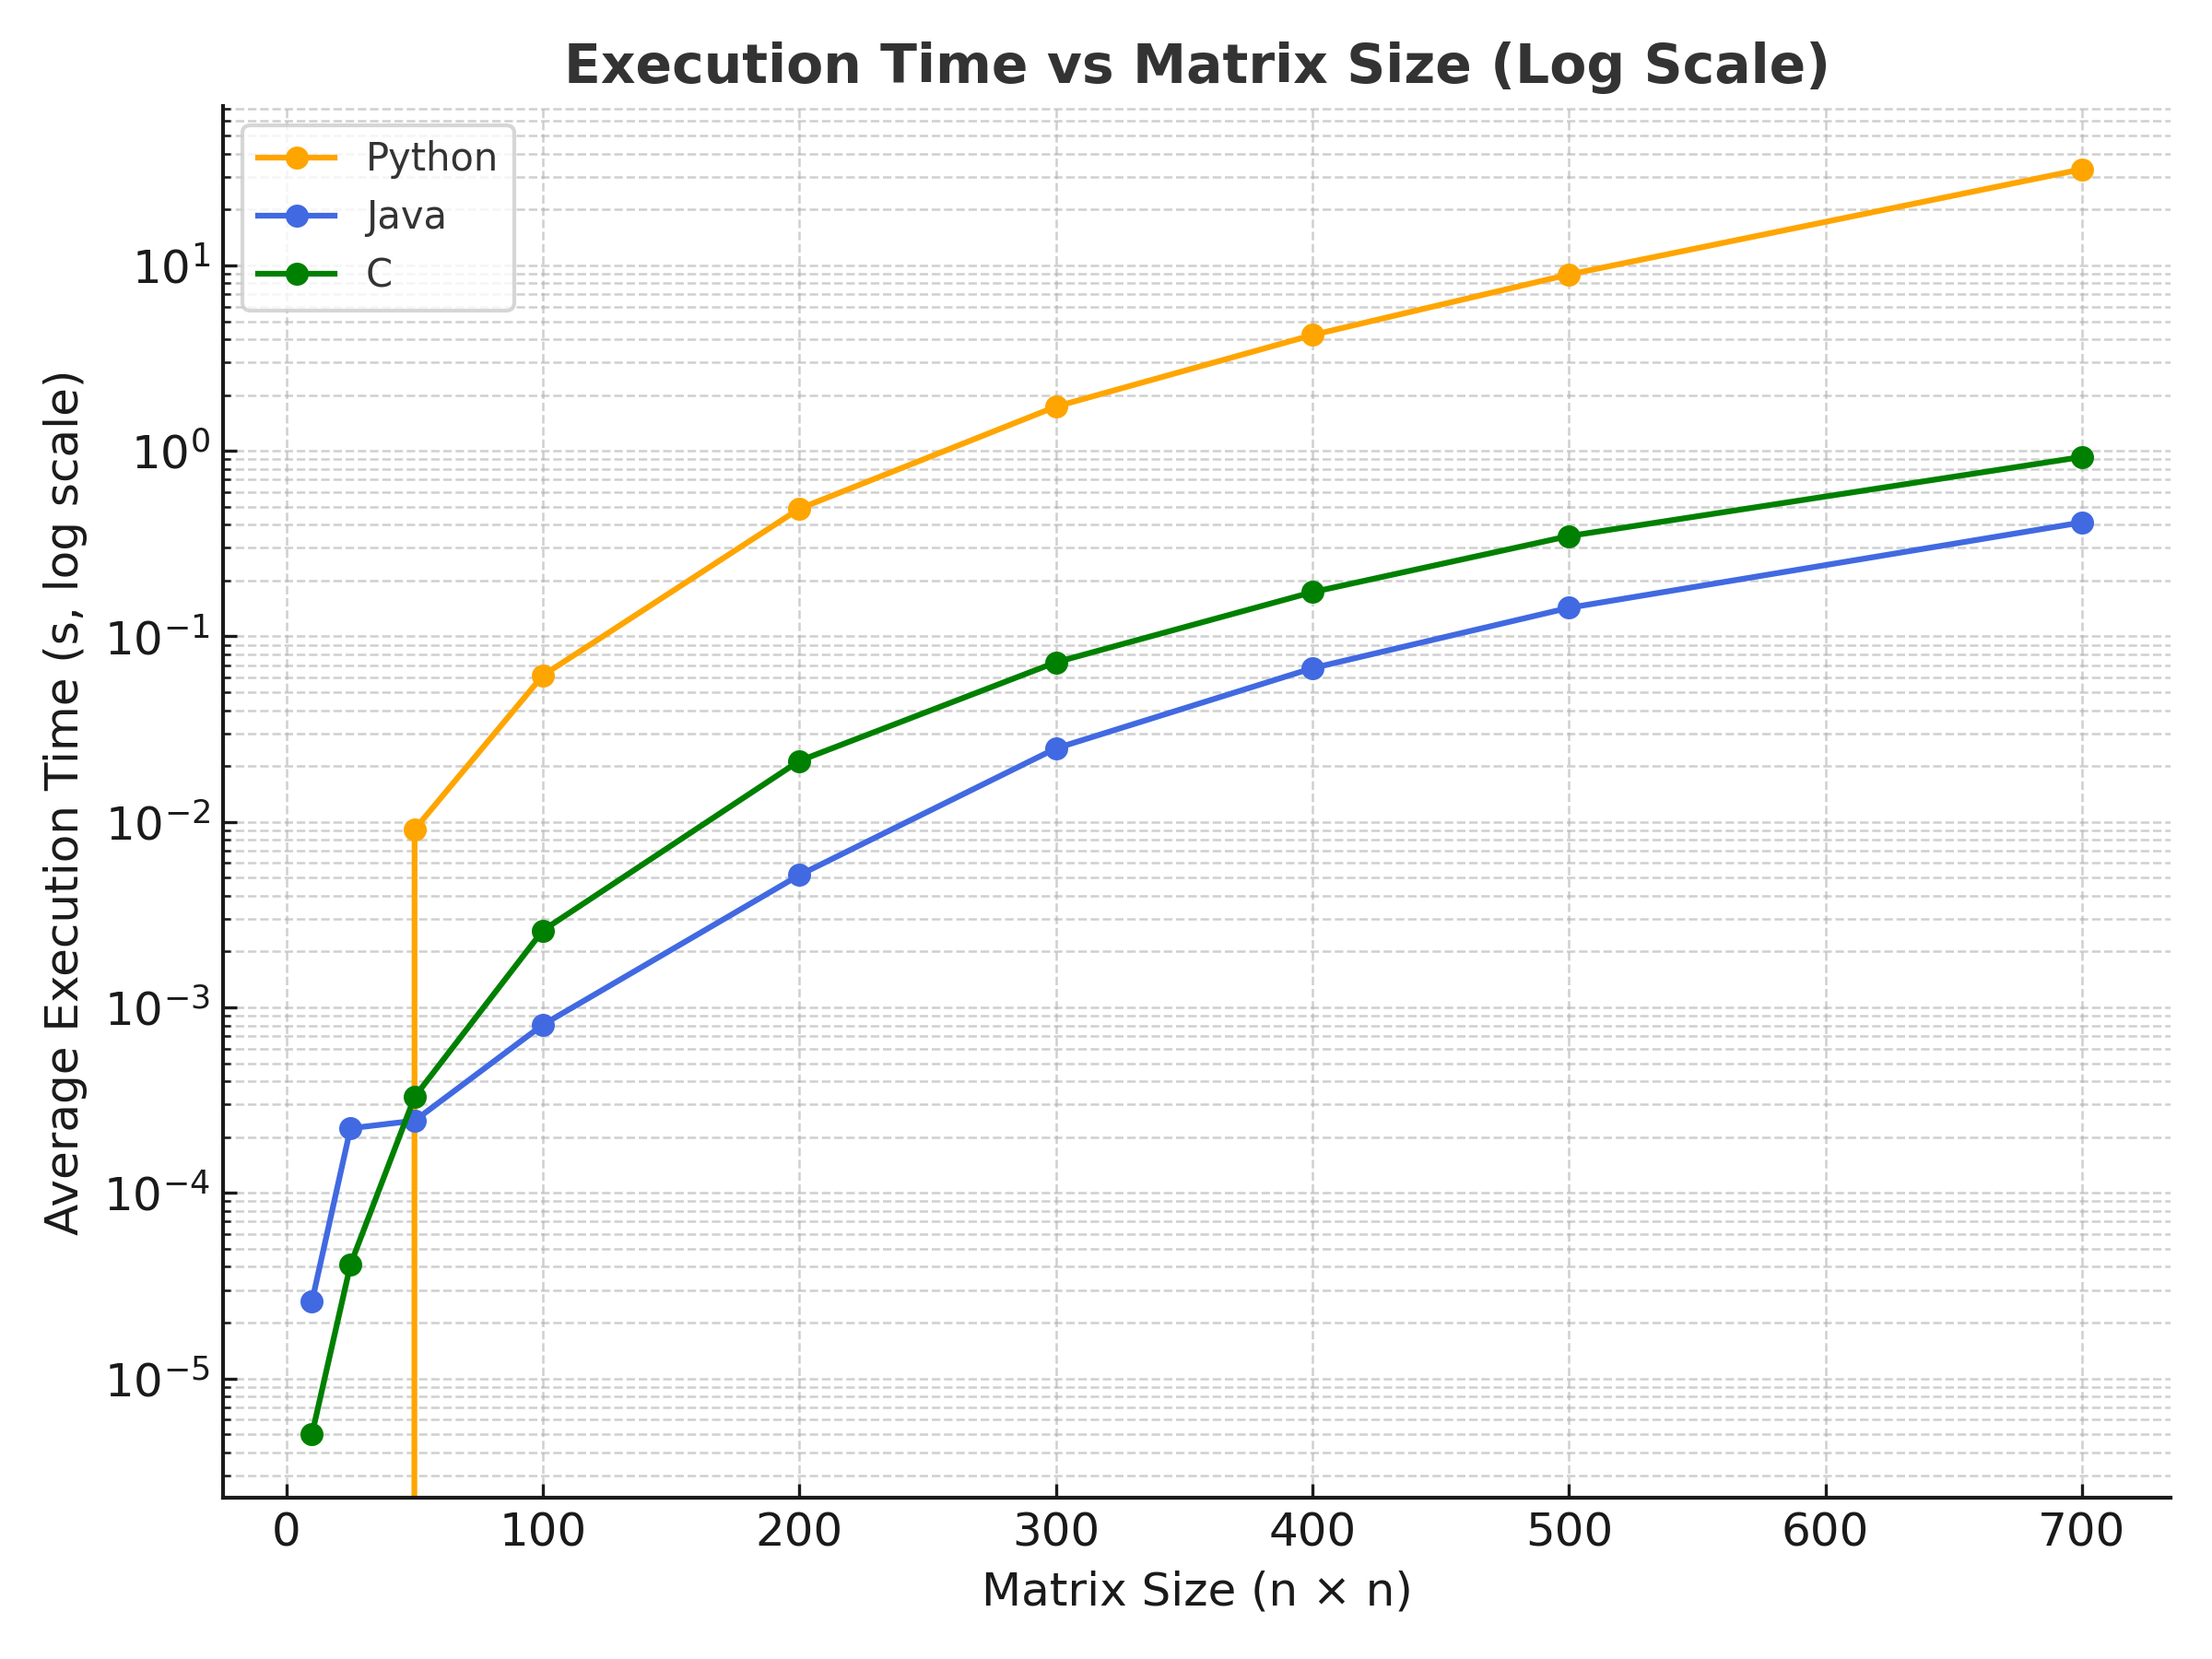
\includegraphics[width=0.85\textwidth]{execution_time_log.png}
    \caption{Execution time comparison using logarithmic scale.}
    \label{fig:log}
\end{figure}
\vspace{2cm} % <-- Más espacio entre la segunda y tercera gráfica
\begin{figure}[H]
    \centering
    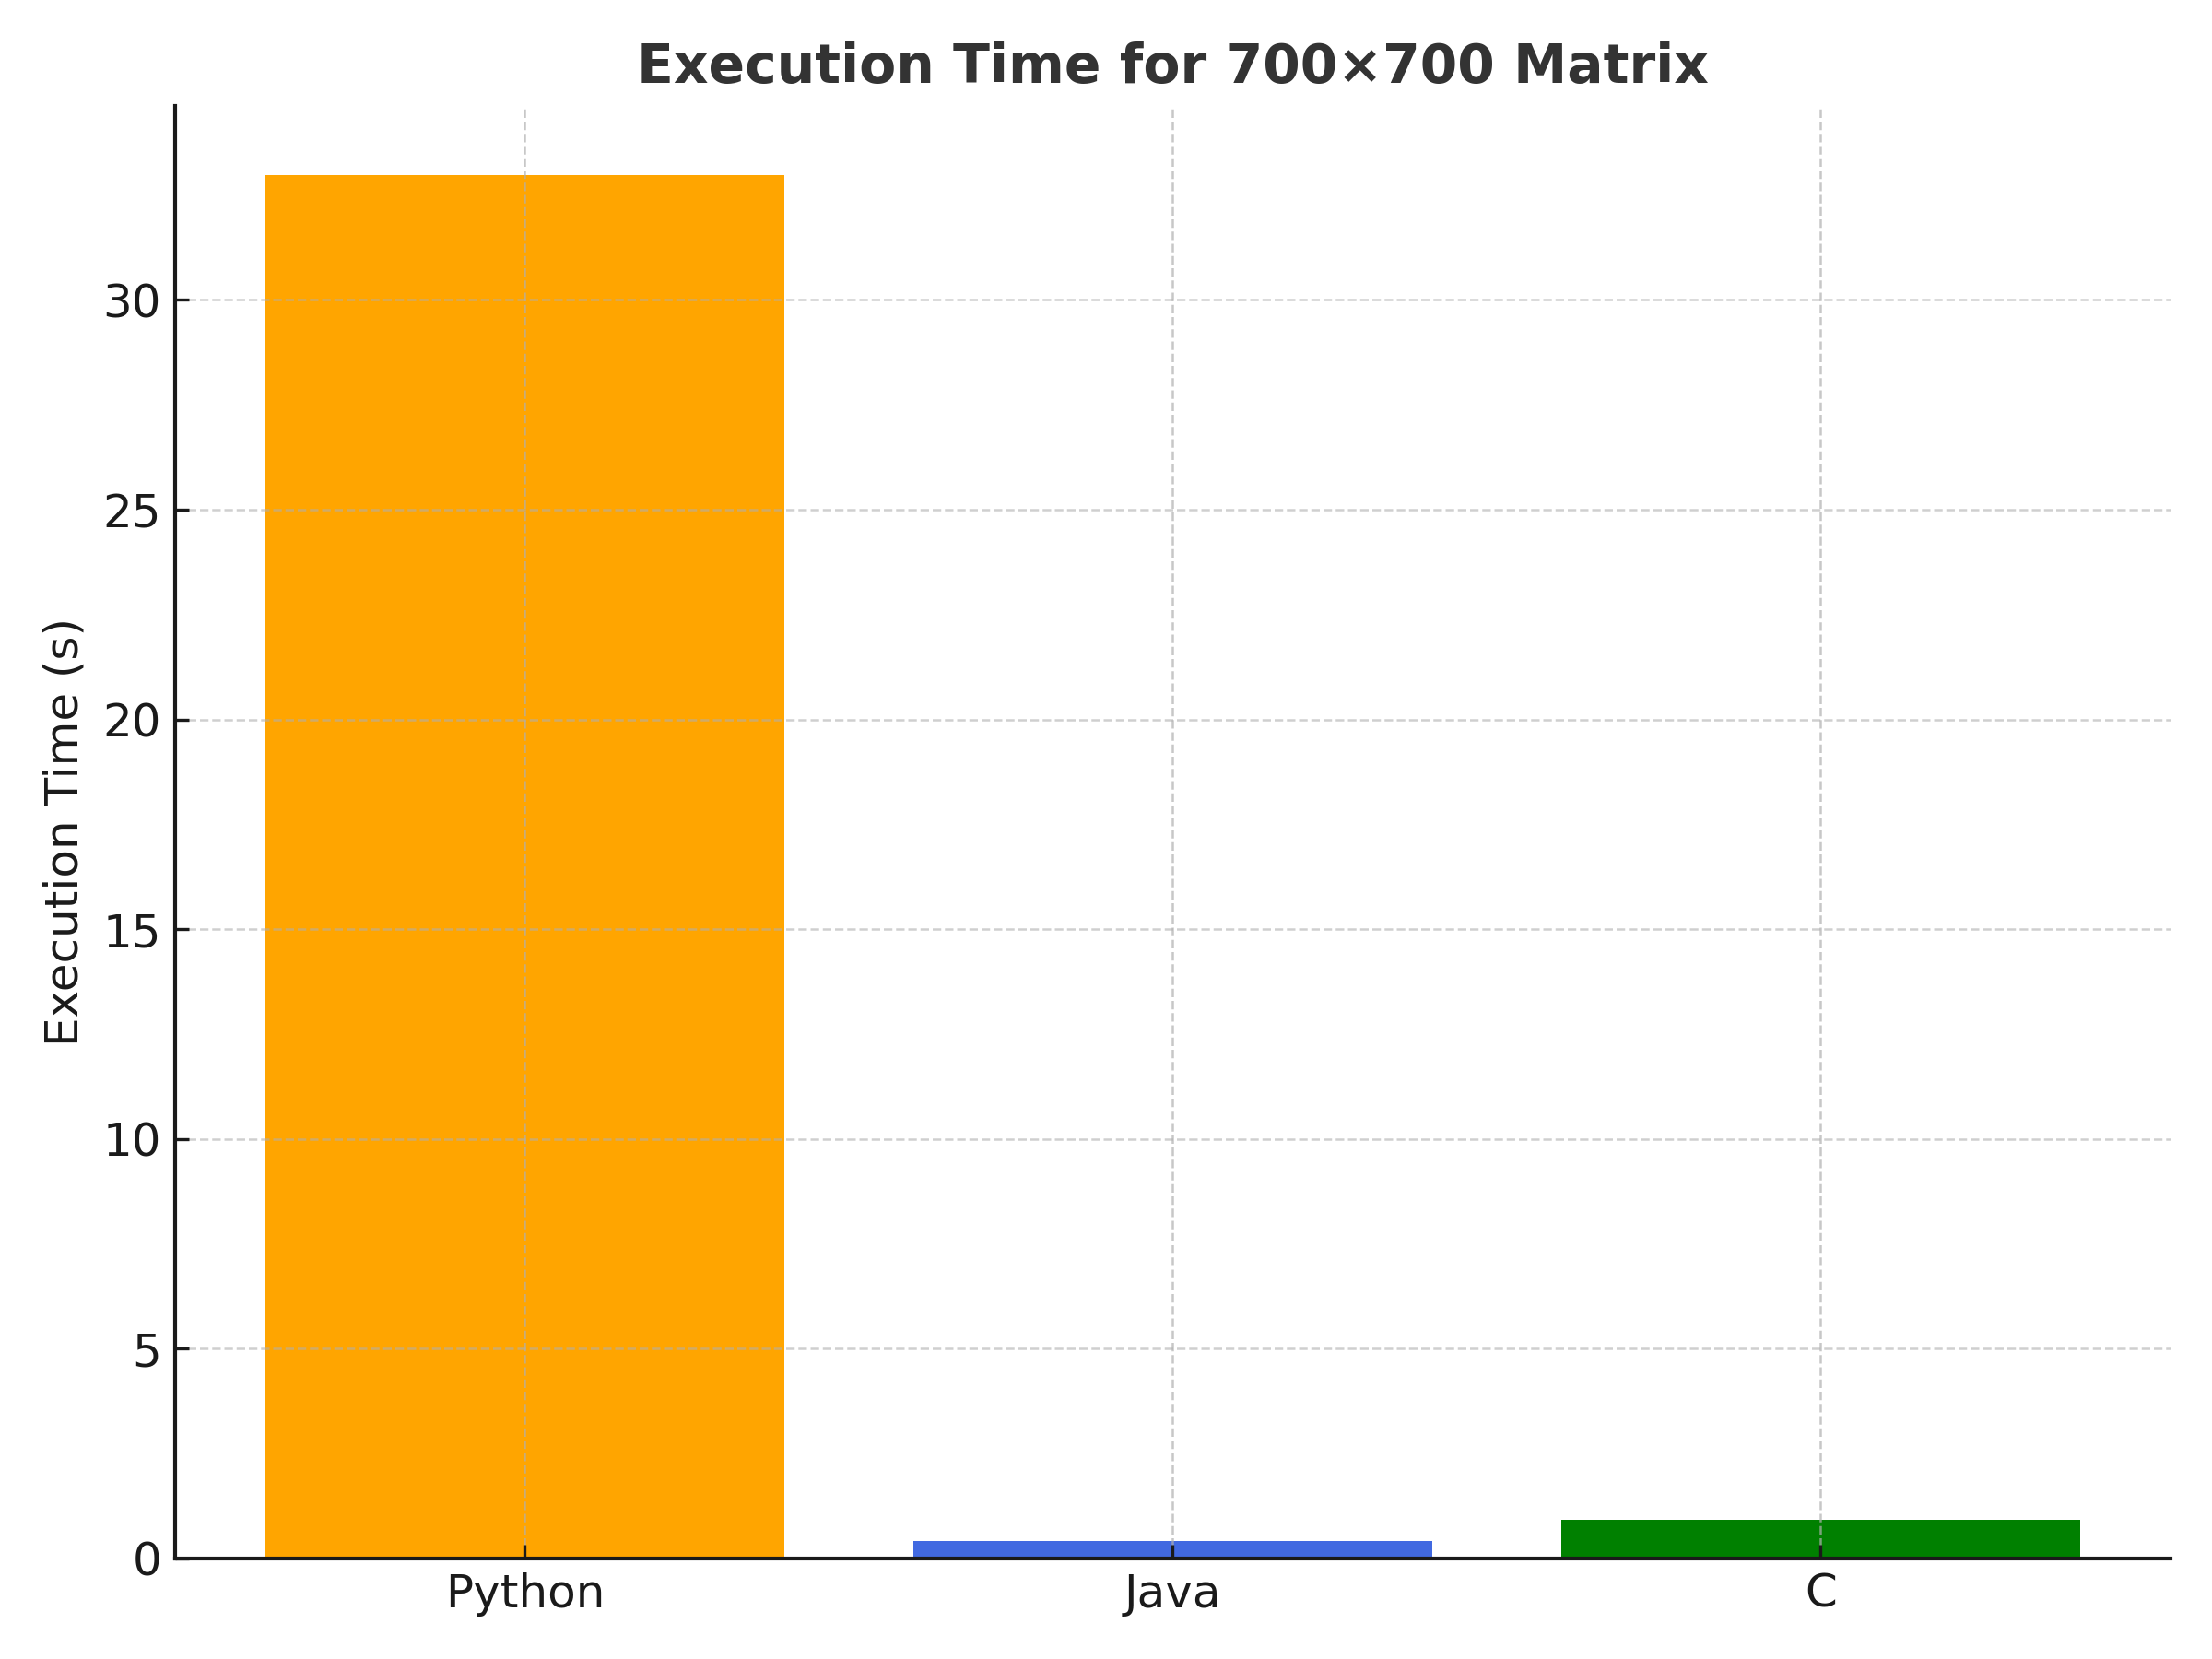
\includegraphics[width=0.7\textwidth]{execution_time_bar.png}
    \caption{Execution time for a 700×700 matrix across programming languages.}
    \label{fig:bar}
\end{figure}

\newpage % <-- Empieza Discussion en una nueva página

\section*{Discussion}

From the results, it is evident that:
\begin{itemize}
    \item \textbf{C} was the fastest language overall, showing the lowest execution times across all matrix sizes. This is expected, given that C is a compiled language that provides direct memory management and minimal runtime overhead.
    \item \textbf{Java} performed slightly slower than C, but still significantly faster than Python. Java benefits from Just-In-Time (JIT) compilation and optimized garbage collection, which contribute to relatively high performance.
    \item \textbf{Python} was considerably slower, especially for larger matrices. As an interpreted language, Python has greater overhead per operation and relies on higher-level abstractions that increase execution time.
\end{itemize}

The logarithmic graph clearly highlights the exponential growth in computation time as matrix size increases, especially for Python. In contrast, both Java and C demonstrate much more stable scaling behavior.

\section*{Conclusion}

This benchmarking study demonstrates the performance gap between compiled and interpreted languages in computationally intensive tasks such as matrix multiplication.

\begin{itemize}
    \item \textbf{C} achieves the best performance and efficiency.
    \item \textbf{Java} offers a good balance between execution speed and ease of use.
    \item \textbf{Python} provides simplicity in development but at the cost of performance.
\end{itemize}

Overall, for large-scale data processing and performance-critical systems, compiled languages such as C or Java are preferable. Python remains useful for prototyping or smaller datasets due to its readability and extensive ecosystem.

\vspace{1cm}
\noindent\textbf{GitHub Repository:} \href{https://github.com/Andrea-Dumpierrez/BigData_Assignment1}{https://github.com/Andrea-Dumpierrez/BigData\_Assignment1}

\end{document}
